% =============================================================================
% P3 --- version revisada (tono TFG). Mantiene el barrido thr x K y el mapa de
% calor como unica figura. Se eliminan presencia_por_captura,
% yolo_rafagas_por_imagen y la matriz de confusion 2x2.
% Figura: presencia_heatmap.png
% =============================================================================
\section{P3 --- ¿Puede el sistema confirmar operativamente la presencia de un dron?}
\label{sec:bloque_presencia}

\subsection{Planteamiento del experimento}
\label{sec:p3_planteamiento}

El recall de caja del \SI{39}{\percent} obtenido en P2 podría sugerir que el sistema solo detecta una de cada tres ráfagas reales. Sin embargo, esa métrica responde a una pregunta de naturaleza distinta a la que plantea una aplicación de vigilancia. La cuestión operativa no es cuántas ráfagas individuales localiza el detector en una imagen, sino si el sistema decide correctamente, para cada ventana de \SI{0.1}{\second}, la presencia o ausencia de un dron en la escena.

Para abordarla se introduce un \emph{clasificador de presencia} a nivel de imagen, definido formalmente en la \cref{sec:implementacion_presencia}: una ventana se declara positiva cuando el número de cajas de clase \emph{drone} con confianza mayor o igual que un umbral $\mathit{thr}$ alcanza al menos un mínimo de~$K$ ráfagas. Esta formulación introduce dos grados de libertad ---el umbral de confianza $\mathit{thr}$ y el número mínimo de ráfagas $K$--- cuyo efecto conjunto sobre el rendimiento se evalúa mediante un barrido sistemático. Se exploran cuatro umbrales de confianza, $\mathit{thr} \in \{0{,}10,\, 0{,}25,\, 0{,}40,\, 0{,}50\}$, y cuatro valores mínimos de ráfagas, $K \in \{1, 2, 3, 4\}$, lo que da lugar a \num{16}~configuraciones evaluadas sobre las \num{600}~imágenes del conjunto de prueba (\num{300} con dron y \num{300} sin dron, en balance exacto).

\subsection{Resultados}
\label{sec:p3_resultados}

La \cref{tab:presencia_sweep} recoge el recall de presencia de las \num{16}~configuraciones. El resultado más destacable es transversal a todas ellas: la precisión y la especificidad valen exactamente \num{1,000} en las dieciséis combinaciones. Es decir, el sistema no declara la presencia de un dron en ninguna de las \num{300}~imágenes de interferencia pura, con independencia del umbral de confianza y del mínimo de ráfagas elegidos. La elección de $(\mathit{thr}, K)$ no introduce falsos positivos; únicamente regula la sensibilidad, esto es, el recall de presencia.

\begin{table}[htbp]
\centering
\caption{Recall de presencia (\%) en función del umbral de confianza $\mathit{thr}$ y del mínimo de ráfagas~$K$. La precisión y la especificidad valen \num{1,000} en las \num{16}~configuraciones.}
\label{tab:presencia_sweep}
\begin{tabular}{lcccc}
\toprule
& \textbf{$K=1$} & \textbf{$K=2$} & \textbf{$K=3$} & \textbf{$K=4$} \\
\midrule
$\mathit{thr}=0{,}10$ & 99,0 & 95,3 & 91,0 & 89,0 \\
$\mathit{thr}=0{,}25$ & 89,0 & 83,0 & 78,3 & 75,3 \\
$\mathit{thr}=0{,}40$ & 82,0 & 76,0 & 71,7 & 70,3 \\
$\mathit{thr}=0{,}50$ & 79,3 & 73,7 & 69,0 & 67,0 \\
\bottomrule
\end{tabular}
\end{table}

La \cref{fig:presencia_heatmap} representa estos valores como un mapa de calor, que facilita la lectura del compromiso entre sensibilidad y exigencia: el recall de presencia es máximo en la esquina superior izquierda (umbral de confianza bajo y pocas ráfagas exigidas) y decrece de forma monótona al endurecer cualquiera de los dos parámetros.

\begin{figure}[htbp]
    \centering
    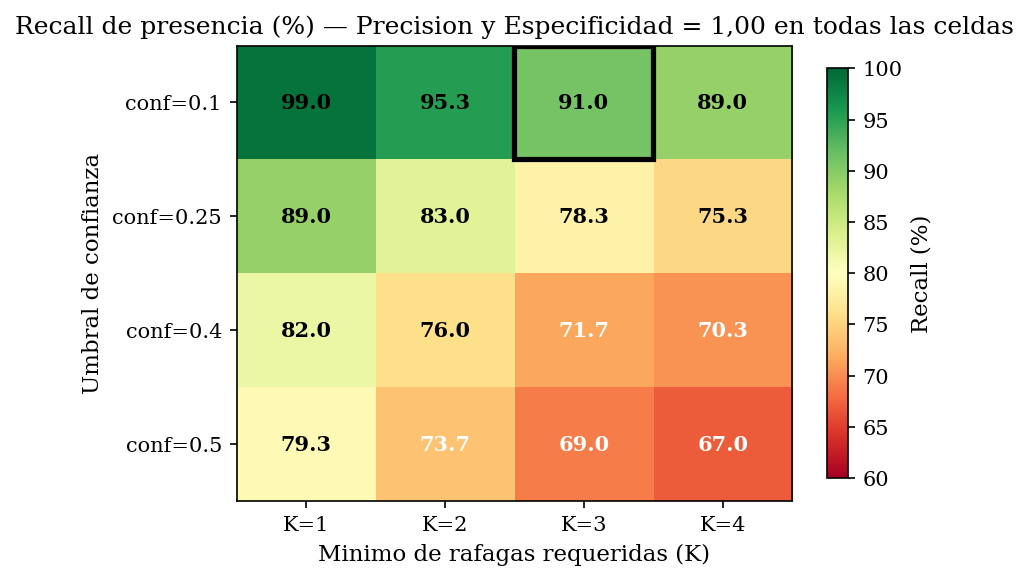
\includegraphics[width=0.70\textwidth]{figuras/resultados/presencia_heatmap.png}
    \caption{Mapa de calor del recall de presencia (\%) en función del umbral de confianza $\mathit{thr}$ y del mínimo de ráfagas~$K$. Las celdas más claras corresponden a mayor recall. El recuadro destacado marca el punto de operación recomendado ($\mathit{thr}=0{,}10$,\, $K=3$), con recall del \SI{91}{\percent} y F1\,=\,\num{0,953}. La precisión y la especificidad valen \num{1,000} en todas las celdas.}
    \label{fig:presencia_heatmap}
\end{figure}

\FloatBarrier
Como punto de operación se adopta $\mathit{thr}=0{,}10$,\, $K=3$, que maximiza el recall de presencia (\SI{91}{\percent}, F1\,=\,\num{0,953}) exigiendo a la vez la coincidencia de tres ráfagas independientes por ventana, lo que protege frente a detecciones espurias aisladas. En este punto, de las \num{300}~ventanas con dron el sistema confirma \num{273} y deja \num{27} sin confirmar (falsos negativos), mientras que las \num{300}~ventanas de interferencia pura se rechazan en su totalidad, sin una sola falsa alarma.


\subsection{Discusión}
\label{sec:p3_discusion}

El resultado central de P3 es la ausencia total de falsos positivos en las \num{16}~configuraciones evaluadas: el sistema no confirma la presencia de un dron en ningún espectrograma que contenga únicamente WiFi y Bluetooth, incluidas las capturas de interferencia más intensa. La precisión y la especificidad perfectas se mantienen con independencia de los parámetros del clasificador de presencia, lo que indica que la decisión positiva del sistema es altamente fiable.

La aparente paradoja entre el recall de caja (\SI{39}{\percent}) y el recall de presencia (\SI{91}{\percent}) se explica por la redundancia temporal del protocolo OcuSync. Una ventana con dron contiene decenas de ráfagas FHSS ---consecuencia directa de un esquema de salto que cambia de canal decenas de veces por cada \SI{0.1}{\second}---, de modo que, aunque el detector falle la mayoría de las ráfagas a nivel individual, le basta con acertar unas pocas para superar el mínimo de $K=3$. El clasificador de presencia actúa así como un agregador que convierte múltiples detecciones débiles en una decisión binaria robusta. En las ventanas sin dron, por el contrario, las detecciones espurias son tan escasas que nunca alcanzan ese mínimo, lo que sostiene la especificidad perfecta.

El análisis por captura matiza el origen de los \num{27}~falsos negativos: se concentran en la captura a \SI{5}{\meter} con WiFi limpio (nivel L1), mientras que la captura a \SI{10}{\meter} con WiFi saturado (nivel L3) se confirma en el \SI{100}{\percent} de sus ventanas. Este comportamiento, contraintuitivo a primera vista, admite una explicación coherente con el protocolo: ante una interferencia intensa, OcuSync tiende a incrementar la densidad de retransmisiones, lo que aumenta el número de ráfagas por ventana y facilita la confirmación de presencia. De ser correcta esta interpretación, el sistema operaría mejor precisamente en el escenario de despliegue más exigente.

Conviene encuadrar el alcance de estas cifras: el barrido se ha realizado sobre el conjunto de prueba del dataset~v3, de carácter interior y controlado (\cref{cap:implementacion}). La especificidad perfecta y el recall del \SI{91}{\percent} son sólidos dentro de ese dominio; su validación sobre un conjunto con mayor diversidad de distancias, niveles de interferencia y entornos ---el dataset~v4 propuesto en el \cref{cap:conclusiones}--- queda planteada como trabajo futuro. En cualquier caso, el punto de operación $\mathit{thr}=0{,}10$,\, $K=3$ constituye un compromiso razonable entre sensibilidad y robustez para una primera versión del sistema de vigilancia.
